\documentclass[11pt,letterpaper]{article}
\usepackage[T1]{fontenc}
\usepackage[utf8]{inputenc}
\usepackage{lmodern,amsmath,amssymb,amsthm,mathtools}
\usepackage[margin=1in]{geometry}
\usepackage{microtype,booktabs,longtable,array,enumitem,xcolor,graphicx}
\usepackage{xurl}
\usepackage[colorlinks=true,linkcolor=blue!45!black,citecolor=blue!45!black,urlcolor=blue!45!black]{hyperref}
\usepackage{fancyhdr}
\pagestyle{fancy}\fancyhf{}
\fancyhead[L]{\small Subexponential SAT: combined bounds and exact code improvements}
\fancyfoot[C]{\thepage}
\setlength{\headheight}{14pt}
\setlength{\emergencystretch}{3em}
\setlength{\parskip}{3pt}
\setlist{itemsep=3pt,topsep=5pt}
\allowdisplaybreaks[2]
\newtheorem{theorem}{Theorem}[section]
\newtheorem{lemma}[theorem]{Lemma}
\newtheorem{proposition}[theorem]{Proposition}
\newtheorem{corollary}[theorem]{Corollary}
\theoremstyle{remark}\newtheorem{remark}[theorem]{Remark}
\newcommand{\poly}{\operatorname{poly}}
\newcommand{\ceil}[1]{\left\lceil#1\right\rceil}
\newcommand{\floor}[1]{\left\lfloor#1\right\rfloor}
\newcommand{\pin}{\texttt{474ddba696a5d385c091c23fb2995f69edd13e00}}
\newcommand{\researchurl}{https://github.com/VladimirReshetnikov/ProveIt/tree/474ddba696a5d385c091c23fb2995f69edd13e00/Computability/SubexponentialSAT/Research}
\newcommand{\incomingurl}{https://github.com/VladimirReshetnikov/ProveIt/tree/474ddba696a5d385c091c23fb2995f69edd13e00/docs/incoming}
\hypersetup{pdftitle={Beyond the combined SAT proposal frontier},pdfauthor={Research prepared for Vladimir Reshetnikov with ChatGPT},pdfsubject={Review of fifteen SAT refinement packets; explicit contraction certificates; exact packet-labeling and precision improvements}}
\title{\textbf{Beyond the Combined SAT Proposal Frontier}\\[5pt]
\large Multi-stage contraction schedules, faster exact labeling,\\
and residual-precision arithmetic}
\author{Research prepared for Vladimir Reshetnikov\\\small with ChatGPT}
\date{October 26, 2026 (Pacific time)}
\begin{document}
\maketitle
\begin{abstract}
We review the seven filed refinement packets in ProveIt's
SubexponentialSAT project, eight second-round packets from
\texttt{docs/incoming}, and their two primary manuscripts. The correct
comparison includes compatible compositions of the newer packing and
Cauchy-mode improvements. We give a multi-stage polynomial-space
contraction schedule with coefficient $63.8522033905\ldots$ on the scale
$s/\sqrt{\log_2s}$, below the composed $66.6051434076\ldots$ certificate
and a strengthened two-stage comparison near $66.1205$. A separately
optimized cached construction gives time coefficient $37.9301090829\ldots$
and space coefficient $33.6230409217\ldots$, below the fixed-alphabet
composed-family time infimum $38.1677456970\ldots$.

Two executable changes complement these mathematical certificates. Caching
row sums in the existing exact packet-labeling implementation reduces its
candidate-scoring phase from $O(NQ^3)$ to $O(NQ^2)$ rational operations,
preserving every score and tie break. Complete certificates agree on 840
cases; the largest of five benchmark fixtures improves from about 304 ms
to 32 ms. An exact valuation-normalization identity moves suitable mode
arithmetic from $P$ bits to $P-V(\beta)$ bits, with an explicit correction
to the creation-precision invariant. Its prototypes pass independent
actual-domain Cauchy checks and show useful arithmetic-kernel savings.

The global SAT logarithmic orders remain unchanged. Numerical coefficients
are per normalized tensor wire, not per SAT variable. The contraction
results retain stated upstream algebraic dependencies; no full SAT solver,
new Lean/Rocq certificate, or end-to-end SAT speedup is claimed.
\end{abstract}
\noindent\textbf{Review pin:} \pin.\\
\textbf{Closing placement reviewed:}
\texttt{6d3adc45061535ebe6fa7cd3d9b37dff7dcfc22a}, October 26, 7:03 pm Pacific.\\
\textbf{Evidence:} source hashes, exact checkers, raw benchmark trials,
reference code, and complete editable report sources accompany this PDF.
\clearpage
\tableofcontents
\clearpage

\section{Results and the comparison standard}
\label{sec:outcome}

The useful outcomes are an actual improvement to a supplied implementation
and smaller explicit contraction certificates after combining the relevant
prior ideas. Merely comparing with the first-round coefficient $648.44$
would miss most of the current frontier.

Let $s$ be the normalized Boolean wire bound, and write
\[
 \mathfrak E(s)=\frac{s}{\sqrt{\log_2s}}.
\]
Suppress fixed polynomial factors in $s$ and the tensor-description length
$\mathcal L$. Table~\ref{tab:frontier} distinguishes polynomial-space
enumeration from the cached algorithm, which spends subexponential space.
The new certificates are proved in Section~\ref{sec:theory}.

\begin{table}[htbp]\centering\small
\caption{Comparable leading exponential certificates. Every time entry
means $2^{(C+o(1))\mathfrak E(s)}$ up to a fixed polynomial. A numerical
space entry has the same interpretation.}
\label{tab:frontier}
\begin{tabular}{@{}p{.58\textwidth}rr@{}}\toprule
Construction or derived comparison & Time $C$ & Space\\\midrule
Best displayed incoming polynomial-space schedule & $76.9090$ & polynomial\\
That schedule with full-block slope-four modes & $66.6051$ & polynomial\\
Strengthened fixed-$16$ boundary comparison & $66.1927$ & polynomial\\
Derived root/tail comparison ($17$, then $13$) & $66.1205$ & polynomial\\
\textbf{New multi-stage schedule} & $\mathbf{63.8522}$ & \textbf{polynomial}\\\midrule
Incoming asymmetric schedule with full-block caching & $44.5376$ & $39.4959$\\
Retuned fixed-$8$ composed-family boundary & $38.1677$ & $33.9927$\\
\textbf{New root-$7$/tail-$9$ cached schedule} & $\mathbf{37.9301}$ & $\mathbf{33.6230}$\\\bottomrule
\end{tabular}
\end{table}

Boundary comparisons are limiting parameter certificates, not empirical
measurements or lower bounds on what the earlier ideas could ever achieve.
The root/tail polynomial-space comparison is an additional compatible
construction derived during this review. None of these numerical searches
is used as a proof of global parameter optimality. The new schedules use
explicit rational parameters and strict packing margins.

The implementation improvement in Section~\ref{sec:packing-code} has a
different evidentiary status: it is benchmarked against a byte-identical
existing implementation and returns the same complete results.
Section~\ref{sec:peeling} gives a second exact transformation and separately
scoped arithmetic-kernel benchmarks. The ratios from these experiments
must not be multiplied by exponent-coefficient ratios to predict a full
SAT speedup.

\subsection{The exact input interface}

The contraction theorems use the interface common to the newer packets.
For fixed constants $A,b,C$, the input is a bipartite Boolean tensor
network with at most $s$ edges, polynomially many vertices, maximum degree
at most $\ceil{s^{9/10}}$, and total description length $\mathcal L$.
Parallel edges are allowed and have distinct ports. Entries belong to
\[
 (\mathbb Z/2^{P_0}\mathbb Z)[V]/(V^\ell),\qquad
 1\le P_0,\ell\le Cs.
\]
Every original entry is evaluable in time
$(s+\mathcal L)^b2^{A s^{9/10}}$ and polynomial space. The extension-ring
arithmetic, deformation, recovery, and recursive factorization are those
of the cited preprint \cite{upstream}, with the refinements explicitly
identified below. The constants in the $o(1)$ terms are uniform for fixed
interface constants. Bounded exceptional sizes can be handled by direct
summation.

\begin{theorem}[The new polynomial-space certificate]\label{thm:ps}
Under this interface and the imported identities stated in
Section~\ref{sec:inherited}, there is a deterministic contraction
construction using polynomial space and time
\[
 (s+\mathcal L)^{O(1)}
 2^{(63.8522033905488\ldots+o(1))\mathfrak E(s)}.
\]
In particular, coefficient $64$ is valid for all sufficiently large $s$.
\end{theorem}

\begin{theorem}[The new cached certificate]\label{thm:cached}
Under the same interface and the imported cached-factorization machinery,
there is a deterministic construction with
\begin{align*}
 T(s,\mathcal L)&\le(s+\mathcal L)^{O(1)}
       2^{(37.9301090829\ldots+o(1))\mathfrak E(s)},\\
 S(s,\mathcal L)&\le(s+\mathcal L)^{O(1)}
       2^{(33.6230409217\ldots+o(1))\mathfrak E(s)}.
\end{align*}
Thus coefficients $38$ and $34$ respectively are valid eventually.
\end{theorem}

These are ordinary mathematical derivations relative to stated imported
lemmas, with independent component review and exact parameter checks.
They are not independently formalized versions of the entire ETH claim.
Their small exponent margins also imply potentially enormous crossover
sizes. The finite timing evidence concerns the two implemented kernels,
not these asymptotic crossovers.

\subsection{What ``all proposals'' can mean rigorously}

The review compares results on the same input and resource interface and
composes compatible improvements before proposing another one. In
particular, the asymmetric packet already counts the fraction $1-1/r$ of
unequal symbols; applying the round-two crossing saving again would be
incorrect. The full-block slope-four basis replaces the older slope-three
basis without changing its family multiplicity. The cached cost must be
re-derived with the new shrinkage and taper schedule rather than scaled
by a ratio taken from a different schedule.

There are two necessary limits to an all-proposals numerical comparison.
The separate Claude manuscript leaves its relevant leading constant
unspecified, so a numerical dominance statement against it is unavailable
\cite{claude}. Several first-round packets state faster logarithmic orders
only under unconstructed algorithmic hypotheses. A finite improvement of
the established $s/\sqrt{\log s}$ coefficient cannot dominate an assumed
$s/\log s$ algorithm as an asymptotic function. We retain those as open
targets. Low-degree specializations are also retained on their stronger
domains rather than compared as if they had the general degree interface.

A portfolio of the applicable established constructions and the new ones
preserves the previous pointwise upper envelopes. For each fixed resource
class, a finite dovetailing has constant-factor scheduling overhead;
alternatively one can choose by their explicit input-dependent guards.
The strict new improvements asserted here concern the displayed common
interface and the actual packet-labeling code. We do not claim to have
optimized every possible recombination of all existing lemmas.

\section{Repository review and provenance}
\label{sec:review}

The closing read-only checkout is pinned to \pin. The initial review used
\texttt{ab2fbc9e03d5c3d0ad6dec8686960bfe498b0b06}, including the seven
ZIPs arriving in \texttt{3e57705c}. The closing check added the matching
packet from \texttt{d098ba43} and reviewed placement commit
\texttt{6d3adc45}, which filed all eight second-round packets under
\texttt{Research}. The earlier commits are \texttt{45233238} (summary of claimed improvements),
\texttt{3e096089} (vendored primary preprint), \texttt{2b925d88}
(placement of the first seven packets), and the arrivals
\texttt{8afdbbea}, \texttt{64b3202e}, and \texttt{a505bd76}
\cite{repo,intake}. A byte comparison confirms all 187 retained relocated
files from the original seven second-round archives are unchanged; the
only additional packet has 24 filed files. The manifest retains initial
and closing identifiers, per-file hashes, and archive members. No remote
repository file was modified.

The repository README explicitly treats the material as external research
and reports no checked ProveIt Lean/Rocq development for this project
\cite{repo}. The current work reads the original reports and relevant
source code rather than treating that README as a proof certificate.
The finite verification performed here applies to the delivered changes;
it does not retrospectively certify every upstream claim.

\subsection{Seven established packets}

\begin{longtable}{@{}>{\raggedright\arraybackslash}p{.25\textwidth}>{\raggedright\arraybackslash}p{.66\textwidth}@{}}
\toprule Packet & Result relevant to the strongest comparison\\\midrule\endfirsthead
\toprule Packet & Result relevant to the strongest comparison\\\midrule\endhead
Factorial Cauchy modes \cite{factorial} &
Integral features with weights $1+j+2v_2(j!)=1+3j-2s_2(j)$;
leading mode coefficient divided by $\sqrt3$. The row offset was already
observed. This is a count/certificate improvement.\\[4pt]
Contraction improvements \cite{contraction} &
Exact taper count, working precision near $6MD/u$, schedule coefficient
$648.4411$, and streamed coefficient extraction. No full solver timing.\\[4pt]
Precision refinement \cite{precision} &
Exact recovery loss and the full-loss taper minimax problem. The optimal
leading scalar loss remains $6M/u$. A stronger structured-summation
algorithm is assumed rather than constructed.\\[4pt]
Uniform density improvement \cite{density} &
Uniform density-sensitive exponent
$\frac n{\sqrt{\log n}}\min\{\log(2+m/n),\log\log n\}$.
Expander and contraction theorems remain imported dependencies.\\[4pt]
Density refinement \cite{density2} &
Overlapping density improvement and precision constants. Contains an
earlier local odd-unit Cauchy Smith profile; that profile is not new here.\\[4pt]
Scalar parity refinement \cite{scalar} &
Exact scalar parity lift, reducing an incidence-degree cap to
$k(p+a-1)$. Faster recursion still needs a missing compact factorization.\\[4pt]
Asymptotic analysis \cite{barriers} &
Explicit barriers for the analyzed mode/taper mechanisms and two missing
interfaces. No stronger unrestricted bound is established.\\\bottomrule
\end{longtable}

The strongest conditional target among these packets is
$2^{O_k(n\log\log n/\log n)}$, with $n/\log n$ at fixed density
\cite{precision}. A smaller index encoding alone does not provide the
required cheap summation or bounded-wire group tensors. The exact taper
minimax result already excludes a further order improvement from merely
retuning that taper. The present work does not rebrand either observation
as a new result.

\subsection{Eight second-round packets, including the closing arrival}

\begin{longtable}{@{}>{\raggedright\arraybackslash}p{.30\textwidth}>{\raggedright\arraybackslash}p{.61\textwidth}@{}}
\toprule Archive family & Contribution and displayed coefficient\\\midrule\endfirsthead
\toprule Archive family & Contribution and displayed coefficient\\\midrule\endhead
Asymmetric balancing \cite{asymmetric} &
Nearly unit padding, separate side degrees, exact crossing fraction,
additive precision buffer; $76.9090$ on the full interface. Its low-degree
specialization has stronger hypotheses. Its annulus slopes tend to three.\\[4pt]
Balanced packing \cite{balanced} &
Deterministic nearly uniform pair loads and capacity scheduling;
$94.7482$. Symmetric degree treatment gives less cumulative capacity.\\[4pt]
High-moment packing \cite{moment} &
Matching/dependency control and an even-moment construction;
$94.7482$. Its $\exp(O(\log^2s))$ setup is paid and is lower order
on the principal scale.\\[4pt]
Matching refinement \cite{matching} &
The closing arrival gives another symmetric matching-potential derivation
of $94.7482$, with fixed alphabet 54 and an adaptive thin-gap schedule.
It does not alter the combined frontier.\\[4pt]
Recursive refinement \cite{recursive} &
A two-level schedule and stronger reciprocal-domain Cauchy weights,
with uniform slope $64/21$; $133.2074$ as displayed. The full-block
slope-four basis is the stronger compatible local ingredient.\\[4pt]
Round-two refinement \cite{roundtwo} &
Matching-potential packing, exact crossing fraction, thin precision gap,
and different root/tail alphabets; $84.0663$. Changing alphabets by depth
is therefore already a prior idea.\\[4pt]
Packet refinement \cite{packet} &
Two-stage pair balancing, near-unit padding, rational schedule, and
additive precision guard; $95.6639$.\\[4pt]
Joint Cauchy modes \cite{joint} &
Group-preserving full-orientation slope-four features at every valuation;
$319.6858$ in its old polynomial-space schedule. Optional cached group
tables and Strassen aggregation give $225.5971$ time and $196.1994$ space
on that schedule. These ingredients must be recomposed with better packing.\\\bottomrule
\end{longtable}

The archive names and exact member paths appear in the source manifest.
The review establishes novelty only relative to this checked corpus.
Classical conditional expectation, Cauchy separation, and Strassen
multiplication are not claimed as inventions of this report. The new
theoretical contribution is the particular capacity-aware multi-stage
and cache-aware schedules, including their complete resource analysis;
the new executable contributions are the two transformations proved below.

\section{Inherited estimates and their compatibility}
\label{sec:inherited}

Let $\lambda=\ceil{\log_2s}$ and let an active call have $M>s/\lambda$
wires. Its packet length is $L=2^a$, its alphabet is $r$, its whole-vertex
label count is $Q=r^a$, and at an active interpolation node of valuation
$i<u$ put $D=2^{a-i}$. In this section $P$ denotes arithmetic precision;
we use $\mathsf B$ for the common padded wire mass.

\subsection{Asymmetric padding and child sizes}

The asymmetric two-stage labeling gives $\mathsf B=(1+o(1))M$ whenever
\begin{equation}\label{eq:packing-gates}
 QR/M=o(1),\qquad Q^2 C\lambda^2/M=o(1),\qquad LQ^2/M=o(1),
\end{equation}
where $R,C$ bound degrees on the two sides \cite{asymmetric}. Its explicit
error under our fixed power gaps is
$\delta_s=O(1/\lambda)+s^{-c+o(1)}$ for a fixed $c>0$. Thus
$\delta_s\log\lambda=o(1)$, which controls accumulated padding through
the recursion; a separate unspecified $o(1)$ at each level would not be
enough to justify a leading coefficient.

At the root both sides have degree at most $\Delta=\ceil{s^{9/10}}$.
At every later call put retained tensors on the row side and fresh packet
tensors on the column side. Then
\begin{equation}\label{eq:side-invariant}
 R_d\le\Delta,\qquad C_d\le2L_{d-1}.
\end{equation}
Every child has at most $2\mathsf B/r$ wires. For valuation $i$, unequal
symbols account for exactly the fraction $1-1/r$ of common padded cells,
giving at most
\begin{equation}\label{eq:families}
 c_i\le\left(2(1-1/r)+o(1)\right)M/D
\end{equation}
families of any one mode index. For a specified directed pair of different
groups the sharper count is
\begin{equation}\label{eq:pair-families}
 c_{gh}\le(2+o(1))M/(r^2D).
\end{equation}
These counts follow from the uniform padded cell arrangement, not from
an independence assumption about the realized labels.

\subsection{Sharp precision with a logarithmic buffer}

The exact Hermite condition count for $q_i=h(u-i)$ is
$hL(2u-2+2^{1-u})$. Taking
\[
 h=\ceil{\frac{M(2L-1)+1}{L(2u-2+2^{1-u})}}
\]
gives enough conditions for deformation degree $M(2L-1)$. The established
safe working allowance is
\begin{equation}\label{eq:precision}
 P_i=p+6hD+hu(a+1),
\end{equation}
where $p$ is inherited precision \cite{contraction,precision}. Use
\begin{equation}\label{eq:buffer}
 b=6\ceil{\log_2\lambda},\qquad
 a_d=\sum_{j=0}^d u_j+(d+1)b,
\end{equation}
and $a_{-1}=0$. At logarithmic depth, inherited precision satisfies
$p=O(s\lambda^2 2^{a_{d-1}})$. Since $i<u_d$,
$D\ge2^{a_{d-1}+b+1}$, whence
\[
 \frac{p}{MD/u_d}=O(\lambda^4 2^{-b})=o(1).
\]
The last jet-evaluation term in \eqref{eq:precision} is also lower order.
Once $u_d\to\infty$ uniformly, $h=(1+o(1))M/u_d$, so
\begin{equation}\label{eq:precision6}
 P_i\le(6+o(1))MD/u_d.
\end{equation}
The schedules below prove that required uniform divergence rather than
assuming it from a fixed-depth calculation.

\subsection{Full-block modes and entropy}

The joint-Cauchy packet proves a finite, group-preserving separation with
integral source features and target weights
\begin{equation}\label{eq:weights}
 w_j=a+1-i+4j-2s_2(j),\qquad 0\le j<D/2,
\end{equation}
where $s_2$ is binary popcount \cite{joint}. It works over the source's
unramified extension, including non-prime residue classes, and retains
the family multiplicity in \eqref{eq:families}. Its normalized triangular
Cauchy factors and their Smith valuations are prior results, not newly
proved here.

Conservatively lower the offset in \eqref{eq:weights} to one and extend
the mode index range. The generating product gives
\[
 \sum_{j\ge0}-\ln(1-e^{-\theta(1+4j-2s_2(j))})
 =\frac{\pi^2}{24\theta}+O(\log^2(2/\theta)).
\]
Combining \eqref{eq:families} and \eqref{eq:precision6} and optimizing
the exponential tilt yields
\begin{equation}\label{eq:local-ps}
 \log_2 N_i\le(K(r)+o(1))\frac{M}{\sqrt{u_d}},\qquad
 K(r)=\frac{\pi\sqrt{2(1-1/r)}}{\ln2}.
\end{equation}
The saddle has $\theta\asymp\sqrt u/D\to0$ uniformly. In particular,
the error relative to the leading bound is
$O((\sqrt u/D)\log^2(D/\sqrt u))=o(1)$, since $D\ge\lambda^6$ and
$u=O(\lambda)$; the ratio is decreasing for sufficiently large
$D/\sqrt u$. All alphabets used below lie in a fixed finite set.

The source's child topology and immutable entry descriptors do not require
the alphabet to be the same at consecutive depths. Labels are freshly
chosen for the current graph. What carries history is the cumulative
packet exponent and the entry creation convention. This validates the
multi-stage compositions while preserving the existing factorization.

\section{New explicit contraction schedules}
\label{sec:theory}

\subsection{Polynomial space: use the side-degree capacity at several depths}

The root pays the symmetric high-degree constraint
$Q_0^2\Delta\ll s$, while subsequent calls need only
$Q_d\Delta\ll s$ for their old side. Their fresh side is much smaller
by \eqref{eq:side-invariant}. The asymmetric packet already exploits this
distinction, and the round-two packet already changes the root alphabet.
Here the cumulative capacity is used at several depths, with progressively
smaller tail alphabets.

Choose the following rational retained-range coefficients:
\begin{equation}\label{eq:ps-schedule}
\begin{array}{c|ccccc}
 d&0&1&2&3&4+k\ (k\ge0)\\\hline
 r_d&13&14&8&6&4\\
 \eta_d&27/2000&51/4000&141/20000&107/20000&(27/6400)(5/8)^k.
\end{array}
\end{equation}
Use $u_d=\floor{\eta_d\lambda}$, the buffer \eqref{eq:buffer}, and leaf
threshold $H=\ceil{s/\lambda}$. All parameters are computable by integer
arithmetic. The cumulative leading ranges are
\begin{equation}\label{eq:ps-capacities}
 A_0=\frac{27}{2000},\quad A_1=\frac{21}{800},\quad
 A_2=\frac{333}{10000},\quad A_3=\frac{773}{20000},\quad
 A_\infty=\frac{499}{10000}.
\end{equation}

\begin{lemma}[Every packing gate has a strict margin]
\label{lem:ps-gates}
At the root, $2A_0\log_2r_0<1/10$. At all later depths,
$A_d\log_2r_d<1/10$. The three conditions in
\eqref{eq:packing-gates} hold uniformly at active logarithmic depths,
and all new tensor degrees stay below $\Delta$.
\end{lemma}
\begin{proof}
The required scalar inequalities have exact integer certificates
\[
 13^{27}<2^{100},\quad 14^{21}<2^{80},\quad
 999<1000,\quad 6^{773}<2^{2000},\quad 998<1000.
\]
They correspond in order to the root and the four tail alphabet regimes.
At the root they give $Q_0^2\Delta=s^{1-c_0+o(1)}$ for fixed $c_0>0$.
Below the root they give $Q_dR_d=s^{1-c_d+o(1)}$ with a uniform positive
minimum margin. The fresh-side exponent satisfies
\[
 2A_d\log_2r_d+A_{d-1}<\frac15+\frac{499}{10000}
 =\frac{2499}{10000}<1.
\]
The same bound controls $L_dQ_d^2$. The added buffers cost only
$O((\log\lambda)^2)=o(\lambda)$ at logarithmic depth, while active
calls have $s/M<\lambda$. These logarithmic factors are absorbed by the
strict power margins. Finally $2L_d=s^{0.0499+o(1)}<\Delta$.
\end{proof}

\paragraph{Noncircular depth argument.}
First prove the preceding estimates for every hypothetical active depth
\[
 d\le\ceil{\log_{5/3}\lambda}+C_0
\]
with a fixed sufficiently large $C_0$. In that range,
\[
 u_d\ge\lambda^{\epsilon_0+o(1)},\qquad
 \epsilon_0=1-\frac{\ln(8/5)}{\ln(5/3)}>0,
\]
where positivity follows from $24<25$. Thus floors are uniformly
negligible, all taper ranges diverge, and the packing and precision
estimates are valid throughout the hypothetical range. For sufficiently
large $s$, every child has at most $3M/5$ wires, because $r_d\ge4$ and
padding tends uniformly to one. No active path can then pass the stated
depth. This establishes the depth bound without assuming the desired
shrinkage before verifying packing.

Using the sharper accumulated padding estimate gives
\begin{equation}\label{eq:ps-size}
 M_d\le(1+o(1))s f_d,
 \quad (f_0,f_1,f_2,f_3)=\left(1,\frac2{13},\frac2{91},\frac1{182}\right),
 \quad f_{4+k}=\frac1{546}\,2^{-k}.
\end{equation}
Apply \eqref{eq:local-ps} and sum the logarithms of branching counts along
a path. The tail work ratio is
$(1/2)/\sqrt{5/8}=\sqrt{2/5}<1$. Therefore the exact leading coefficient is
\begin{align}
 C_{\rm ps}={}&\frac{K(13)}{\sqrt{27/2000}}
 +\frac{2K(14)}{13\sqrt{51/4000}}
 +\frac{2K(8)}{91\sqrt{141/20000}}\notag\\
 &+\frac{K(6)}{182\sqrt{107/20000}}
 +\frac{K(4)}{546\sqrt{27/6400}\,(1-\sqrt{2/5})}.
 \label{eq:ps-constant}
\end{align}
The exact rational interval checker proves
\begin{equation}\label{eq:ps-interval}
 63.85220339054<C_{\rm ps}<63.85220339056<64.
\end{equation}
It uses rational bounds from Machin's arctangent formula for $\pi$, a
positive series for $\ln2$, and integer-square-root brackets. A
floating-point parameter search suggested the schedule but is not an
input to the proof.

Polynomial choices of interpolation node, residue-field evaluation, and
child group over $O(\log\lambda)$ levels contribute
$O(\lambda\log\lambda)$ to the logarithm of total work. Leaf summation
costs $2^{O(s/\lambda)}$. Original entry oracles cost
$2^{O(s^{9/10})}$; new packet entries cost at most
$\exp(O(L_d\log s))=\exp(s^{0.0499+o(1)})$. All are lower order than
$\mathfrak E(s)$. Polynomial-bit descriptions, arithmetic and precision,
together with depth-first traversal, preserve polynomial space. The
description-length factor stays a fixed polynomial because branching
depends on $s$, not on $\mathcal L$. This proves
Theorem~\ref{thm:ps}.

\subsection{A stronger comparison than the displayed prior coefficients}

The incoming asymmetric schedule uses $r=16$, root range $\lambda/81$,
and a geometric tail of the same total range. Composing it with full-block
modes multiplies its slope-three coefficient by $\sqrt3/2$, giving
$66.6051434076\ldots$. Its fixed-alphabet capacity boundary and optimal
tail allocation give the stronger derived value
\begin{equation}\label{eq:prior-fixed}
 K(r)\sqrt{20\log_2r}
 \left[1+\frac{2/r}{(1-(2/r)^{2/3})^{3/2}}\right],
\end{equation}
which at $r=16$ is $66.1927236936\ldots$.

For a root alphabet $r_0$ and a constant tail alphabet $r_1$, set
\[
 x_0=\frac{.05}{\log_2r_0},\qquad
 U=\frac{.1}{\log_2r_1}-x_0>0.
\]
The corresponding optimally allocated geometric tail has coefficient
\[
 \frac{K(r_0)}{\sqrt{x_0}}+
 \frac{(2/r_0)K(r_1)}{\sqrt U\,(1-(2/r_1)^{2/3})^{3/2}}.
\]
At $(r_0,r_1)=(17,13)$ it is about $66.12047546$. These formulas give
feasible limiting comparisons by introducing a vanishing reserve in the
capacities; they do not assert global minima over all schedules. The new
strict rational coefficient in \eqref{eq:ps-interval} is below all three
comparisons. Its gain is about $4.13\%$ against the direct composed
certificate and $3.43\%$ against the stronger root/tail comparison.

\subsection{Cached contraction: pay for the group functions}
\label{sec:cache-theory}

The cached method is inherited from the joint-Cauchy packet \cite{joint}.
Partition a mode tuple by its exact total weight on every directed pair
of groups. With fixed $r$ and polynomial precision, there are only
polynomially many weight arrays, although the polynomial degree can be
large. For one array, let $h_e$ be the base-two logarithm of the number
of exact-weight tuples on pair $e$. Polynomial-size dynamic programming
over modes and weights supplies exact counts and rank/unrank operations;
an efficient hidden oracle is not assumed.

Put
\begin{equation}\label{eq:cache-K}
 \kappa=\frac{\pi\sqrt2}{\ln2},\qquad
 \mathcal K(M,u)=\kappa\frac{M}{\sqrt u}.
\end{equation}
From \eqref{eq:pair-families}, the slope-four generating function, and
the global weight budget, the common-tilt argument gives for fixed
nonnegative pair weights $z_e$,
\begin{equation}\label{eq:weighted-entropy}
 \sum_ez_e h_e\le
 \left(\sqrt{\frac{\sum_ez_e^2}{r^2}}+o(1)\right)\mathcal K(M,u).
\end{equation}
Using one common tilt matters: it includes zero and small individual
weight budgets without incorrectly applying a separate large-budget
asymptotic to each pair.

Cache each group's function of its incident pair indices, obtaining
each value by a genuine recursive child contraction. Partition the
groups into three blocks. Sum internal indices to form block boundary
tables, then contract the resulting triangle using division-free
rectangular Strassen multiplication. For block size $k$, the numbers
of incident and boundary directed pairs are respectively
\[
 I_r(k)=2rk-k^2-k,\qquad J_r(k)=2k(r-k).
\]
If the three inter-block classes have sizes $v_1,v_2,v_3$, the rectangular
matrix exponent follows from
\[
 H_1+H_2+H_3-(3-\omega)\min(H_1,H_2,H_3),\qquad \omega=\log_2 7.
\]
Writing this as the maximum of three weighted sums and using
\eqref{eq:weighted-entropy} gives the matrix coefficient
\begin{equation}\label{eq:matrix-b}
 b_r=\sqrt{\frac{v_1+v_2+v_3-[1-(\omega-2)^2]\min_jv_j}{r^2}}.
\end{equation}
The cache, block-construction, and memory coefficients are
\begin{equation}\label{eq:cache-factors}
 a_r=\frac{\sqrt{2(r-1)}}r,\qquad
 B_r=\max\left\{b_r,\frac{\sqrt{\max_k I_r(k)}}r\right\},\qquad
 j_r=\frac{\sqrt{\max_k J_r(k)}}r.
\end{equation}
Here $B_r$ must include both block-table construction and matrix work.
Omitting the former would be a mistake for the root schedule below.

Up to the already controlled polynomial and lower-order factors, the
correct recurrence is
\begin{equation}\label{eq:cache-recurrence}
 T_d\le2^{a_{r_d}\mathcal K_d}\,r_dT_{d+1}
           +2^{B_{r_d}\mathcal K_d}.
\end{equation}
Thus caching does not grant free group tensors. The first term pays for
all recursive evaluations, and the second pays for the tables and their
contraction. The inherited sequential-record implementation, reblocking
and sorting show that polynomial overhead suffices in a bit-cost model;
an exponential random-access table is not treated as a unit-cost oracle.
Strassen uses only additions, subtractions and multiplications, so it is
valid in the source's residue ring with nilpotents.

\subsection{Why the stronger fixed-alphabet baseline must be included}

At the asymmetric packet's displayed $r=16$ schedule, the new per-pair
counts and full-block cached method give time coefficient
$44.5375718550\ldots$ and space coefficient $39.4959495337\ldots$.
But one can retune the existing fixed-alphabet family. At $r=8$, root
capacity $x_0=1/60$, and a tail of the same total capacity, the appropriate
recurrence is root dominated for a range of geometric tail allocations.
Its limiting time coefficient is
\begin{equation}\label{eq:r8-baseline}
 C_{8,\partial}=\kappa\sqrt{60}
  \sqrt{\frac{30+12(\omega-2)^2}{64}}
  =38.1677456970\ldots,
\end{equation}
with space coefficient $33.9927010637\ldots$. Vanishing capacity reserve
handles the equality boundary. This is the more demanding comparator
used here, rather than only the $44.54$ displayed-schedule composition.

\subsection{The new strict root-7/tail-9 schedule}

Use seven groups at the root, partitioned as $(2,2,3)$, and nine groups
at every later depth, partitioned as $(3,3,3)$. Set
\begin{equation}\label{eq:new-cache-schedule}
 \eta_0=\frac{89}{5000},\qquad
 \eta_d=\frac{1233}{125000}\left(\frac7{25}\right)^{d-1}\quad(d\ge1),
 \qquad u_d=\floor{\eta_d\lambda}.
\end{equation}
Keep the buffer \eqref{eq:buffer} and $H=\ceil{s/\lambda}$.
The tail total is $137/10000$, and the total cumulative capacity is
\[
 A_\infty=\frac{89}{5000}+\frac{137}{10000}
 =\frac{63}{2000}=0.0315.
\]
The exact inequalities
\begin{equation}\label{eq:cache-gates}
 7^{89}<2^{250},\qquad 9^{63}<2^{200}
\end{equation}
give the strict root gate $2\eta_0\log_2 7<1/10$ and tail gate
$A_\infty\log_2 9<1/10$. The fresh-side and padding exponents are
less than $1/5+A_\infty=0.2315<1$. New tensor degrees are at most
$s^{0.0315+o(1)}<\Delta$.

Verify these bounds first through hypothetical depth
$\ceil{\log_4\lambda}+O(1)$. Tail ranges satisfy
\[
 u_d\ge\lambda^{1-\ln(25/7)/\ln4+o(1)}\longrightarrow\infty
\]
because $25/7<4$. Eventually the root child shrinkage is at most $1/3$
and every tail child shrinkage at most $1/4$, while the sharp factors
are $2/7$ and $2/9$ respectively. This closes the same noncircular
depth bootstrap as before and validates the uniform precision estimates.
Accumulated padding errors give
\[
 M_0\le s,\qquad
 M_d\le(1+o(1))s\frac27\left(\frac29\right)^{d-1}\quad(d\ge1).
\]

Write $\xi=\omega-2=\log_2(7/4)$. At the root,
\begin{equation}\label{eq:root-cache-factors}
 a_7=\frac{\sqrt{12}}7,\quad
 b_7=\frac{\sqrt{24+8\xi^2}}7,\quad
 B_7=\frac{\sqrt{30}}7,\quad j_7=\frac{\sqrt{24}}7.
\end{equation}
Here $b_7<B_7$: root block construction costs more than root matrix
multiplication. In the tail,
\begin{equation}\label{eq:tail-cache-factors}
 a_9=\frac49,\quad
 B_9=b_9=\frac{\sqrt{4+2\xi^2}}3,\quad j_9=\frac23.
\end{equation}
The tail block-construction coefficient $\sqrt{42}/9$ is smaller than
$B_9$. The tail work ratio is
\begin{equation}\label{eq:cache-gamma}
 \gamma=\frac{2/9}{\sqrt{7/25}}=\frac{10}{9\sqrt7}<1.
\end{equation}
Moreover $a_9/(1-\gamma)=0.766231\ldots<B_9=0.767655\ldots$.
This strict inequality ensures that all deeper cache evaluations are
covered by the first tail node's local table bound.

Let
\[
 K_0=\frac{\kappa}{\sqrt{89/5000}},\qquad
 K_1=\frac{(2/7)\kappa}{\sqrt{1233/125000}}.
\]
Unrolling \eqref{eq:cache-recurrence}, the normalized total time
coefficient is at most
\begin{equation}\label{eq:cache-final}
 C_{\rm cache}=\max\{B_7K_0,\ a_7K_0+B_9K_1\}
 =a_7K_0+B_9K_1.
\end{equation}
The root table term is $37.59170256\ldots$; the second term, including
recursive child work, is $37.9301090829\ldots$ and is the bottleneck.
The memory coefficient is
\begin{equation}\label{eq:cache-memory}
 C_{\rm mem}=\max\{j_7K_0,j_9K_1\}=j_7K_0
 =33.6230409217\ldots.
\end{equation}
Ancestor and descendant table sizes add, so their leading space exponents
take a maximum, rather than a sum. There are only logarithmically many
stack levels, and the tail $\mathcal K_d$ decreases geometrically.

The supplied checker proves these comparisons with rational intervals,
including a positive margin in $a_9/(1-\gamma)<B_9$ and the complete
root maximum. It encloses
\begin{align*}
 37.93010908288&<C_{\rm cache}<37.93010908289<38,\\
 33.62304092165&<C_{\rm mem}<33.62304092167<34.
\end{align*}
The same lower-order costs already checked for Theorem~\ref{thm:ps}
are harmless here, with an even smaller packet exponent. This proves
Theorem~\ref{thm:cached}. The time coefficient improves by about $0.62\%$
over \eqref{eq:r8-baseline}; the comparison is a strict improvement of
certificates, not a prediction of a $0.62\%$ runtime reduction.

\subsection{Consequences for SAT and the unresolved order improvement}

Let $n$ be the declared variable count, $m$ the number of clauses and
$k$ a fixed width. The unchanged reduction and the density refinements
give the polynomial-space envelope
\begin{equation}\label{eq:sat-envelope}
 (n+m)^{O_k(1)}\,
 2^{O_k\left(\frac n{\sqrt{\log n}}
      \min\{\log(2+m/n),\log\log n\}\right)}.
\end{equation}
Small sizes are understood with the usual harmless logarithm offsets.
At fixed density this is $2^{O_{k,D}(n/\sqrt{\log n})}$ up to polynomial
factors. At unrestricted density it has the
$n\log\log n/\sqrt{\log n}$ numerator/denominator profile. The new
engine preserves these orders and improves its specified wire-level
certificate. Converting it to a numerical coefficient per variable
requires the reduction's actual wire and width constants. In particular,
writing $2^{64n/\sqrt{\log n}}$ as a universal SAT consequence would
be unsupported.

The cached version can use the same reductions at its different space
cost. Direct clause-network bounds and prior low-degree specializations
remain options in a portfolio. The separate manuscript's unspecified
constants cannot be ranked numerically from the supplied information.

The persistent obstacle to a smaller logarithmic order is unchanged:
the mode weights still grow linearly, their weighted partitions have
the $M/\sqrt u$ entropy scale, and packing keeps $u=O(\log s)$.
The existing scoped barriers do not prove a lower bound for SAT; they
show why the present retuning and exact arithmetic transformations do
not establish $n/\log n$ or eliminate the dense reduction's extra
$\log\log n$. A further order improvement still requires an actual
summation/factorization interface or a different representation,
with its oracle and wire costs paid explicitly.

\section{A faster implementation of the existing balancing algorithm}
\label{sec:packing-code}

The most direct performance result is an optimization of code already in the
reviewed repository. It changes neither the mathematical labeling algorithm
nor its output. The reference is the asymmetric packet's
\texttt{code/balanced\_packing.py} \cite{asymmetric}; a byte-identical copy is
included as \texttt{code/reference\_balanced\_packing.py}. The source already
caches products involving unassigned columns. Our improvement also caches
the row sums used to score every candidate label.

\subsection{Exact conditional expectations}

After the deterministic greedy row labeling, let $Q$ be the number of
labels and let $w_{av}$ be the number of edges from row-label class $a$ to
column vertex $v$. Let $X_{ab}$ be the loads from columns assigned so far.
The reference uses the rational base
\[
 z=1+\frac1{h\max(1,C)},
\]
where $C$ is the maximum column degree and $h\ge2$ is the smoothness
parameter. For each row-label class, define
\[
 F_a=\prod_{v\ \mathrm{unassigned}}\frac{Q-1+z^{w_{av}}}{Q},
 \qquad S_a=\sum_{b=0}^{Q-1}z^{X_{ab}}.
\]
The exact conditional expectation is $\Phi=\sum_a F_aS_a$.
Before assigning column $v$, remove its factor:
\[
 F'_a=F_a\left(\frac{Q-1+z^{w_{av}}}{Q}\right)^{-1}.
\]
All these are ordinary positive rational numbers. They are unrelated to
the nonunit divisions in the two-adic contraction ring.

\begin{proposition}[Cached candidate scores]
\label{prop:scores}
The conditional expectation after assigning $v$ to label $b$ is exactly
\begin{equation}\label{eq:score}
 \Phi_b=\underbrace{\sum_a F'_aS_a}_{B}
       +\sum_a F'_a(z^{w_{av}}-1)z^{X_{ab}}.
\end{equation}
After selecting $b_*$, update
\[
 S_a\leftarrow S_a+(z^{w_{av}}-1)z^{X_{ab_*}},\quad
 z^{X_{ab_*}}\leftarrow z^{X_{ab_*}}z^{w_{av}},\quad
 F_a\leftarrow F'_a.
\]
Every score, its minimizing label with the original tie rule, and the
conditional-expectation certificate are identical to the reference.
\end{proposition}
\begin{proof}
Only cell $(a,b)$ changes when $v$ receives label $b$. Its contribution
to $S_a$ changes from $z^{X_{ab}}$ to $z^{X_{ab}+w_{av}}$.
Subtract the former from the latter and factor the difference to obtain
\eqref{eq:score}. The displayed updates preserve the definitions of $S_a$,
the cell powers, and $F_a$. Induction over columns proves equality with
the reference computation. Since the rational scores are exactly equal,
their ordering, all ties, and the selected labels are equal as well.
\end{proof}

For $N$ column vertices, the reference loops over $Q$ candidate labels,
$Q$ row classes, and $Q$ column classes per assignment. Its candidate-score
phase costs $O(NQ^3)$ rational operations. Formula~\eqref{eq:score} computes
the common base once and uses a $Q$-term correction for each of $Q$ labels,
giving $O(NQ^2)$ rational operations. The additional cell-power cache has
$Q^2$ rational entries. Greedy row assignment, the adjacency scan, and
the shared table of powers $z^0,\ldots,z^M$ remain unchanged. For example,
with $R_0$ input row vertices, a direct overall arithmetic count is
\[
 O(M+R_0N+R_0Q+(N+1)Q^2)
\]
for the new implementation, with $NQ^3+Q^2$ in place of $(N+1)Q^2$ for
the reference's scoring and cell bookkeeping. These are rational-operation counts;
the cost of multiplying long integer numerators and denominators must
still be paid. All operands have the same polynomial bit-length envelope
as in the original method. We do not assert a factor-$Q$ bit-time
speedup on every input.

\subsection{Comparison with the actual reference code}

The verification program compares complete returned objects, including
every exact potential, selected label, cell load, and certificate string.
It passed 840 full-certificate comparisons, covering 9,724 candidate scores;
840 additional comparisons with certificate storage disabled; and 12
invalid-input checks. A normal Python run and an optimized
\texttt{python -O} run give identical verification records. The checks use
explicit exceptions, so optimization does not remove them.

Table~\ref{tab:packing-bench} gives five paired timing trials per instance,
alternating which implementation runs first. Both retain their exact
internal averaging and final-potential checks. Both disable only the
serialization of certificate histories for the timing run. The recorded
JSON includes all trial times and the actual adjacency matrices, permitting
replay without relying on an unspecified input generator.

\begin{table}[htbp]\centering
\caption{Measured packet-labeling times. These are comparisons of the
existing subroutine and its exact replacement, not full SAT timings.}
\label{tab:packing-bench}
\begin{tabular}{@{}rrrrr@{}}\toprule
Rows $\times$ columns & $Q$ & Reference (ms) & Cached (ms) & Ratio\\\midrule
$12\times16$ & 4 & 1.652 & 1.100 & $1.50$\\
$16\times24$ & 8 & 10.974 & 4.111 & $2.67$\\
$20\times32$ & 12 & 39.088 & 9.140 & $4.28$\\
$24\times40$ & 16 & 103.253 & 18.320 & $5.64$\\
$24\times40$ & 24 & 304.464 & 31.833 & $9.56$\\\bottomrule
\end{tabular}
\end{table}

The benchmark is a small, seeded collection on one execution host, using
the recorded Python version and standard-library \texttt{Fraction}
arithmetic. Five repetitions do not establish a cross-machine performance
distribution. The implementation-level saving is nevertheless directly
testable: it performs fewer exact score computations and returns the same
objects as the faster relevant prior implementation. It is suitable for
integration independently of the proposed new asymptotic schedules.

\section{Precision peeling for mode contributions}
\label{sec:peeling}

The source retains a mode tuple $\beta$ when its guaranteed valuation
$V(\beta)=\sum_z w_z\beta_z$ is below the working precision $P$.
It then passes precision $P$ to its child contractions. A further exact
transformation removes those guaranteed powers of two before computing
the contribution. Its correctness does not require a new Cauchy basis,
a particular recursion schedule, or a probabilistic model of the tensor.

\subsection{The algebraic identity}

Use the source's integral coefficient ring
$\mathcal A=\mathcal O[V]/(V^\ell)$, with all congruences interpreted
coordinatewise. Freeze the current tensor entries at their specified
creation-time representatives. Write every targeted mode coefficient as
$c_{xz}=2^{w_z}\bar c_{xz}$, where $\bar c_{xz}\in\mathcal A$.
The affine row factors include local terms $a_x$ and the appropriate signs
from $l_0(t)=1-t$ or $l_1(t)=t$.

\begin{lemma}[Exact coefficient normalization]\label{lem:normalization}
For every multi-index $\beta$,
\begin{equation}\label{eq:normalization}
 [Z^\beta]\prod_x\left(a_x+\sum_zc_{xz}Z_z\right)
 =2^{V(\beta)}[Z^\beta]
       \prod_x\left(a_x+\sum_z\bar c_{xz}Z_z\right).
\end{equation}
\end{lemma}
\begin{proof}
The left polynomial is obtained from the right polynomial by substituting
$Z_z\mapsto2^{w_z}Z_z$. Coefficient comparison gives the identity. It
remains true with cancellations, nilpotent coordinates, and zero terms.
No equality between the valuation of a sum and the minimum valuation of
its summands has been assumed.
\end{proof}

Normalize each packet/group tensor by the contribution of the modes it
targets, leaving source moments unchanged. Let $v_g(\beta)$ be the sum
of target valuations in group $g$. Multilinearity of contraction gives
$Z_{g,\beta}=2^{v_g(\beta)}\bar Z_{g,\beta}$. Every mode has exactly
one target, hence $\sum_gv_g(\beta)=V(\beta)$.

\begin{theorem}[Residual precision]\label{thm:peeling}
For every retained tuple define $Q(\beta)=P-V(\beta)>0$. The recursive
mode identity may be evaluated as
\begin{equation}\label{eq:peeling}
 F(t+\alpha\zeta)\equiv
 \sum_{V(\beta)<P}2^{V(\beta)}
       \prod_g\bigl(\bar Z_{g,\beta}\bmod2^{Q(\beta)}\bigr)
       \pmod {2^P}.
\end{equation}
The normalized children use the same graph and ports. Tuples with
$V(\beta)\ge P$ require no child contraction.
\end{theorem}
\begin{proof}
Apply Lemma~\ref{lem:normalization} separately in every packet and group,
then substitute in the existing exact factorization. Replacing each
normalized factor by its residue modulo $2^Q$ changes its product by a
multiple of $2^Q$. The outside factor $2^V$ makes that error a multiple
of $2^P$. Addition of contributions preserves the congruence.
\end{proof}

\subsection{Division and creation-time representatives}

Two details are essential for a valid implementation. First, to obtain
$\bar c_{xz}$ modulo $2^Q$, compute $c_{xz}$ modulo $2^{Q+w_z}$ and
divide its canonical coordinates by $2^{w_z}$ as ordinary integers.
Alternatively, cancel the known powers in the exact factored formula and
invert only units. Dividing a residue known only modulo $2^Q$ would lose
$w_z$ output bits. For every used mode, $\beta_z>0$ implies $w_z\le V$,
so $Q+w_z\le P$: the original precision already supplies the needed
information. Unused modes can be omitted from that coefficient extraction.

Second, residual precision can decrease along a recursive path. The
source's original implementation assumes increasing precision and freezes
creation-time representatives \cite{upstream}. Therefore the normalized
child must be a newly specified network at precision $Q$. Reduce each
retained parent representative modulo $2^Q$ and freeze the resulting
canonical residue; create normalized packet entries at $Q$ as well.
Later lifting uses these new representatives. It must not return to an
older, larger representative or reevaluate an unfrozen defining formula.

A retained descriptor can carry a precision cap. Further caps flatten
to their minimum, because canonical reductions modulo powers of two
compose. This avoids a growing stack of evaluator wrappers. An older
entry evaluator may still run at its original creation precision before
its result is capped. The theorem does not promise to reduce that cost.

In the cached algorithm, each outer exact-weight array fixes the total
$V$. Consequently $Q=P-V$ is fixed throughout that array, and its entire
triangle multiplication can use the same ring $\mathcal A/(2^Q)$.
Thus peeling is compatible with caching; it does not require adding
quantities from different residue rings in a single matrix product.

\subsection{What arithmetic work can be saved}

Let $N(t)$ count feasible tuples with $V<t$; additional fixed support or
degree constraints may be included. The total precision charge for one
linear-in-precision operation per contribution has the exact identity
\begin{equation}\label{eq:layercake}
 \sum_{V(\beta)<P}(P-V(\beta))=\sum_{t=1}^P N(t)
 \le P N(P).
\end{equation}
To prove it, write each positive integer $P-V$ as a sum of $P-V$ ones
and exchange the two finite sums. More generally, for nondecreasing $f$
with $f(0)=0$,
\begin{equation}\label{eq:generalcharge}
 \sum_{V(\beta)<P} f(P-V(\beta))
 =\sum_{q=1}^P\bigl(f(q)-f(q-1)\bigr)N(P-q+1).
\end{equation}
These are operation-charge identities, not wall-clock predictions.

There is also a useful certified upper estimate. Put
$\mathcal Z(\theta)=\prod_z(1-e^{-\theta w_z})^{-1}$ for positive weights.
For any $\alpha>0$ and $\theta>0$,
\begin{equation}\label{eq:tilted-work}
 \sum_{V(\beta)<P}(P-V(\beta))^\alpha
 \le\left(\frac{\alpha}{e\theta}\right)^\alpha
       e^{\theta P}\mathcal Z(\theta).
\end{equation}
Indeed $q^\alpha e^{-\theta q}\le(\alpha/(e\theta))^\alpha$ for $q>0$,
and extending the remaining sum to all tuples gives $\mathcal Z$.
For the same tilted counting certificate, full precision contributes
$P^\alpha e^{\theta P}\mathcal Z(\theta)$. The ratio of these two upper
certificates is $(\alpha/(e\theta P))^\alpha$.
At the contraction saddle, $\theta P\asymp M/\sqrt u$, giving a
polynomial prefactor saving in this specified arithmetic model.
This is not a ratio of actual runtimes, nor a proof that all oracle work
scales with residual precision.

An exact dynamic program for four colored families of weights
$5+4j-2s_2(j)$ at $P=1024$ gives mean residual precision about $25.04$
bits and linear precision-charge ratio $0.02445$. This is an abstract
infinite-family partition inventory truncated by the budget, not an
assertion that one particular finite packet has that distribution.
Finite packet lengths and active valuation levels must still be supplied
when using the model for a concrete network.

Peeling leaves the number of mode tuples unchanged. Moreover the existing
global schedules make the next Hermite loss dominate the inherited
precision. The present argument therefore does not decrease the leading
$s/\sqrt{\log s}$ entropy term by itself. Its useful scope is arithmetic
that is actually moved to the smaller residue ring.

\subsection{Executable evidence}

The self-contained prototype checks 544 randomized cyclic tensor
contractions, including 120 terms vanishing by valuation. It also compares
18 mode contractions of actual permissible Cauchy subblocks with direct
original-kernel sums at precisions from 8 through 80, rejects four invalid
normalizations, and runs 1,601 canonical-cap regressions. Normal and
optimized Python runs agree. The actual-domain test uses an independent
exact rational elimination to reconstruct the relevant Cauchy block,
rather than importing the prior feature implementation.

Table~\ref{tab:peeling-bench} measures a separate arithmetic kernel:
the cyclic contraction of five dense $12\times12$ matrices, with input
precision $P=2048$ bits and controlled total divisibility $V$.
Both methods receive the same frozen canonical inputs. The peeled time
includes validation and normalization; input generation is excluded from
both timings. Seven paired trials alternate execution order.

\begin{table}[htbp]\centering
\caption{Synthetic cyclic-contraction speed ratios, including normalization.
These quantify an arithmetic kernel, not a complete SAT algorithm.}
\label{tab:peeling-bench}
\begin{tabular}{@{}rrr@{}}\toprule
Removed bits $V$ & Residual precision $Q$ & Full/peeled median time\\\midrule
0 & 2048 & $0.99$\\
512 & 1536 & $1.63$\\
1024 & 1024 & $3.11$\\
1536 & 512 & $6.63$\\
1792 & 256 & $9.48$\\
1984 & 64 & $14.34$\\\bottomrule
\end{tabular}
\end{table}

The zero-valuation row records the small overhead when there is no
precision to remove. The other rows show why the transformation can be
useful, while leaving open the frequency and cost share of such operations
in a complete implementation. All trial times, seeds, dimensions, and
environment metadata are retained in the accompanying JSON.

\begin{figure}[htbp]\centering
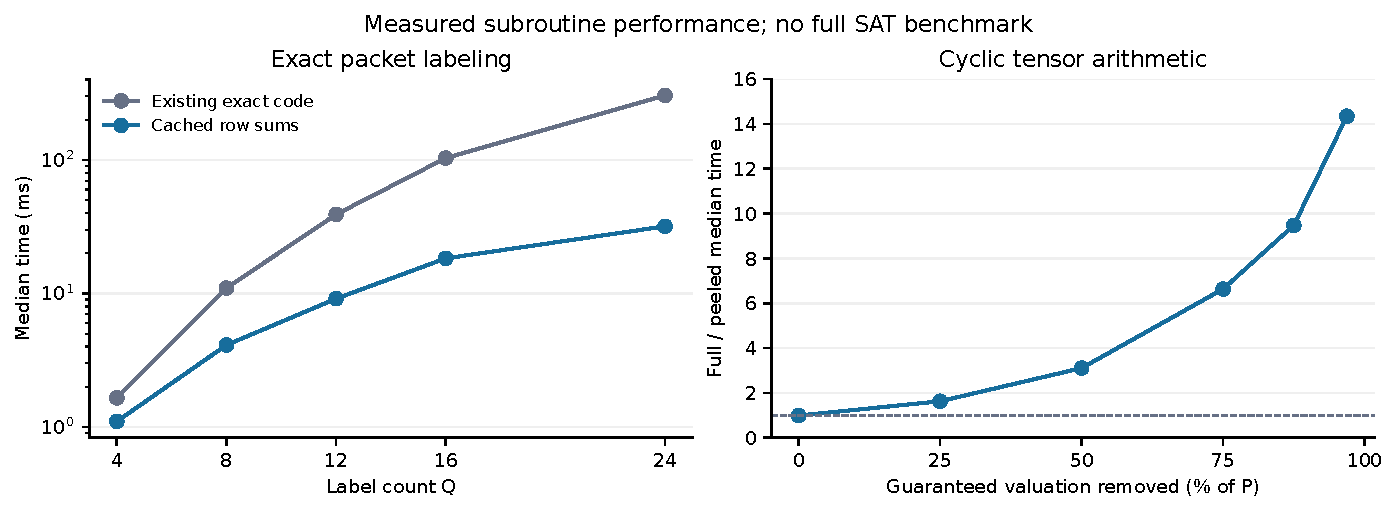
\includegraphics[width=\textwidth]{figures/kernel_benchmarks.pdf}
\caption{Two distinct measured improvements. Left: the existing exact
labeling code versus its cache-preserving replacement. Right: full-precision
versus normalized cyclic matrix contraction. The panels have different
workloads and should not be multiplied into a predicted SAT speedup.}
\label{fig:benchmarks}
\end{figure}

\section{Reproduction, integration, and proof status}
\label{sec:delivery}

\subsection{What the archive contains}

The report's complete editable source is \texttt{report.tex}, with
\texttt{theory.tex}, \texttt{implementation.tex}, \texttt{delivery.tex},
and \texttt{references.tex}. The compiled \texttt{report.pdf} is included.
The \texttt{code/} directory contains the two implementations, the
byte-identical reference labeling routine, exact checkers, benchmark
drivers, and a script to regenerate the figure from the recorded JSON.
The benchmark results retain raw trials and input data. The mathematical
checkers use Python's standard library only; regenerating the figure
also requires Matplotlib. Building the PDF requires a standard LaTeX
installation with the packages listed in its preamble.

The \texttt{provenance/} directory records the checkout commit, relevant
commits, source hashes, archive members, and the reference implementation's
license. The \texttt{notes/} directory retains the detailed review and
independent proof-checking notes. Those are research records rather than
additional verified theorems. The manifest records every delivered file
except the manifest itself. It establishes bundle consistency, not an
independent signature or provenance authority.

\subsection{Replay}

From the extracted archive directory:
\begin{verbatim}
python3 run_checks.py
python3 code/benchmark_cached_balancing.py --output new_packing_times.json
python3 code/benchmark_precision_peeling.py --output new_precision_times.json
python3 code/make_figures.py
python3 build_report.py
\end{verbatim}
On a Windows installation, \texttt{py} may replace \texttt{python3}.
The first command runs all four correctness/parameter checkers normally
and with optimization enabled, compares their parsed results, and writes
a release-verification summary. The benchmark commands deliberately write
new files so the recorded measurements remain intact. Their wall-clock
values depend on the execution host and load.

\subsection{Integration order}

The smallest independently usable change is replacing the asymmetric
packet's \nolinkurl{balance_pair_labels} implementation with
\texttt{cached\_balancing.py}. It preserves the call signature and returned
object. Its exact comparison suite can serve as a migration regression.
This does not require adopting a new contraction schedule.

For the polynomial-space mathematical construction, retain the source
deformation, group factorization and immutable tensor descriptions. Use
asymmetric balancing, the prior full-block Cauchy modes, the exact taper,
the buffer \eqref{eq:buffer}, and schedule \eqref{eq:ps-schedule}.
Keep separate degree bounds for retained and fresh sides; replacing them
by one maximum would discard the extra capacity used in the proof.

The cached construction is a separate resource option. Use schedule
\eqref{eq:new-cache-schedule}, exact directed-pair weight arrays, the
specified root/tail block partitions, and recurrence
\eqref{eq:cache-recurrence}. Compute group functions by recursive
contraction. Pay for block construction as well as matrix multiplication.
Do not quote a cache gain as if the group values were free.

Finally, precision peeling can be applied inside either mode-summation
method. Normalize target coefficients before the precision reduction,
freeze each new child's capped representatives, and restore the outside
power $2^V$ when accumulating modulo $2^P$. The cap regression in the
checker shows why retaining an older larger representative during a later
lift would give the wrong semantics. This change is appropriate only
where those representatives and divisions are handled explicitly.

\begin{longtable}{@{}>{\raggedright\arraybackslash}p{.40\textwidth}>{\raggedright\arraybackslash}p{.51\textwidth}@{}}
\toprule Claim or component & Evidence and boundary\\\midrule\endfirsthead
\toprule Claim or component & Evidence and boundary\\\midrule\endhead
New multi-stage coefficient below 64 &
Ordinary proof of gates, precision, recurrence and space; exact rational
certificate; independent analytic review. Imported contraction lemmas remain dependencies.\\[4pt]
New cached coefficients below 38 and 34 &
Complete paid recurrence, block/table counts and memory proof; exact
interval checks; independent review including the root table term.\\[4pt]
Faster exact labeling implementation &
Algebraic score identity; exact equality to supplied reference on 840
instances; raw paired benchmark trials. This is an implemented subroutine.\\[4pt]
Residual-precision identity &
Exact coefficient substitution and congruence proof, valid in the full
integral ring; implementation and actual-domain checks over rational scalars.
No new extension-ring implementation is supplied.\\[4pt]
Full upstream ETH theorem &
Imported framework; not independently formalized or rebuilt here. The
repository and preprint are identified precisely.\\[4pt]
Full fast SAT program or measured SAT acceleration &
Not supplied. Local code and timing evidence must not be presented as a
full formula-to-count implementation.\\[4pt]
Smaller unrestricted logarithmic order &
Not established. The missing structured-summation or representation
interfaces in the earlier packets remain open.\\\bottomrule
\end{longtable}

\subsection{Where another substantial gain would need to come from}

The delivered changes remove redundant work while preserving established
invariants. The direct engineering next step is integrating the exact
labeling replacement and residual-precision representation into a complete
contraction engine, then measuring their share of actual time. That would
answer a question these isolated kernels cannot: whether packing,
coefficient extraction, creator-oracle evaluation, or mode enumeration
dominates at usable sizes.

For a mathematical order improvement, the concrete missing target is
still a mode-summation or compression algorithm with controlled group
tensor evaluation cost. The local full-block Smith profile grows linearly,
so another invertible integral basis change within that same block cannot
make its invariant-factor growth quadratic. That local statement leaves
open cancellation across modes, a different deformation, and a more
economical SAT-to-network representation. A future claim along any of
those routes should specify the actual interface and account for its
precision, wire count, oracle cost, and memory before comparing exponents.

\appendix
\section{Independent elementary bounds for the cached headline}

The interval checker gives many more digits than the theorem needs. For
a short independent certificate, let $\xi=\log_2(7/4)$. Exact integer
powers give
\[
 \frac{25}{31}<\xi<\frac{13}{16},\qquad
 7^{31}>2^{87},\quad 7^{16}<2^{45}.
\]
The tail ratio satisfies $\gamma<21/50$, so
\[
 \frac{a_9}{1-\gamma}<\frac{200}{261}
 <\frac{\sqrt{566}}{31}<B_9.
\]
For the total coefficient, rational brackets from the positive logarithm
series and Machin's formula give
\[
 \kappa<6.413,\qquad
 \frac{a_7}{\sqrt{89/5000}}<3.710,\qquad
 \frac{(2/7)B_9}{\sqrt{1233/125000}}<2.213.
\]
Their products imply
\[
 C_{\rm cache}<6.413(3.710+2.213)=37.984199<38.
\]
Similarly $j_7/\sqrt{89/5000}<5.250$, hence
$C_{\rm mem}<33.66825<34$. All square-root comparisons reduce to
integer inequalities after squaring positive quantities. The full
independent review also verifies that the first-tail cached-child term
exceeds the root table term. The supplied exact interval checker proves
all the corresponding strict comparisons directly.

\section{Source-to-change map}

\begin{longtable}{@{}>{\raggedright\arraybackslash}p{.43\textwidth}>{\raggedright\arraybackslash}p{.48\textwidth}@{}}
\toprule Original source location & Use or replacement\\\midrule\endfirsthead
\toprule Original source location & Use or replacement\\\midrule\endhead
Preprint quantitative contraction: coefficient ring and exact arithmetic &
Retain integral extension arithmetic and immutable representative semantics.
For peeling, add the explicit creation cap of Section~\ref{sec:peeling}.\\[4pt]
Preprint packet-packing lemma &
Use the incoming asymmetric lemma and preserve its uniform padded-cell
arrangement; optionally run the faster exact scorer.\\[4pt]
Preprint tapered Hermite recovery &
Use the already established exact condition count and six-unit leading
precision allowance. The additive buffer remains necessary.\\[4pt]
Preprint crossing-mode expansion &
Use the joint packet's full-orientation slope-four features, retaining
one source and one target group per mode.\\[4pt]
Preprint child networks and implicit descriptions &
Retain the graph topology and creator descriptors. Track fresh-side degree
separately when applying the new schedules.\\[4pt]
Joint packet's exact pair-index mode graph &
Use its computed group caches and division-free rectangular multiplication,
with new alphabets and the full new recurrence.\\[4pt]
Asymmetric packet's executable column scoring &
Replace repeated row summation by Proposition~\ref{prop:scores}; the
returned labeling and exact certificate remain identical.\\\bottomrule
\end{longtable}

\begin{thebibliography}{99}
\raggedright
\bibitem{repo} Vladimir Reshetnikov and ProveIt contributors.
\emph{Sub-exponential 3-SAT project index}, reviewed at commit
\nolinkurl{474ddba696a5d385c091c23fb2995f69edd13e00}.
\url{https://github.com/VladimirReshetnikov/ProveIt/tree/474ddba696a5d385c091c23fb2995f69edd13e00/Computability/SubexponentialSAT}.

\bibitem{intake} ProveIt, \emph{New research report(s)}, commit
\nolinkurl{3e57705cf14ee9ac99c0ac35cfff751dcf70b396}, October 26, 2026.
\url{https://github.com/VladimirReshetnikov/ProveIt/commit/3e57705cf14ee9ac99c0ac35cfff751dcf70b396}.
Seven incoming archives are identified by filename and SHA-256 in the
accompanying \nolinkurl{provenance/source_manifest.json}. Closing arrival
\nolinkurl{d098ba436b33df19365a44dd178694ff52845d19} adds the matching packet;
placement commit \nolinkurl{6d3adc45061535ebe6fa7cd3d9b37dff7dcfc22a}
files all eight second-round packets:
\url{https://github.com/VladimirReshetnikov/ProveIt/commit/6d3adc45061535ebe6fa7cd3d9b37dff7dcfc22a}.

\bibitem{upstream} OpenAI, \emph{The Exponential Time Hypothesis is False},
October 25, 2026. Preprint sources pinned to
\nolinkurl{7ef5c0cc5ca4b0e072b7a050fca09ab24bc6fa3a}, especially
\nolinkurl{build/quantitative-contraction.tex} and
\nolinkurl{build/quantitative-reduction.tex}.
\url{https://github.com/openai/math/tree/7ef5c0cc5ca4b0e072b7a050fca09ab24bc6fa3a/preprints/The-Exponential-Time-Hypothesis-is-False-October-25-2026}.
The reviewed byte-identical vendored copy is recorded in ProveIt's
\nolinkurl{lib/openai-math/preprints/PROVENANCE.md}.

\bibitem{claude} \emph{A $2^{o(n)}$ time algorithm for 3-SAT}, credited
to Claude (Anthropic), October 26, 2026. The separate 49-page manuscript
filed as \nolinkurl{Research/claude-2o-n-3sat/eth.pdf}; retrieved from the
pinned ProveIt project. Its reported proof development was not supplied
for independent execution in this review.

\bibitem{factorial} \emph{Cauchy mode improvement}, October 26, 2026.
ProveIt \nolinkurl{Research/cauchy_mode_improvement/report.tex} and
associated code. Integral factorial features and mode-count analysis.

\bibitem{contraction} \emph{ETH contraction improvements}, October 26,
2026. ProveIt \nolinkurl{Research/eth_contraction_improvements/report.tex},
with schedule and finite-difference extraction artifacts.

\bibitem{precision} \emph{3SAT precision refinement}, October 26, 2026.
ProveIt \nolinkurl{Research/3sat_precision_refinement/report.tex}.
Exact recovery loss, taper minimax calculation, and conditional
structured-summation target.

\bibitem{density} \emph{Density-aware SAT improvement}, October 26, 2026.
ProveIt \nolinkurl{Research/sat_density_improvement/}
\nolinkurl{density_aware_sat_improvement.tex}.

\bibitem{density2} \emph{ETH density refinement}, October 26, 2026.
ProveIt \nolinkurl{Research/eth_density_refinement/report.tex}.
Density-sensitive bounds and local Cauchy arithmetic.

\bibitem{scalar} \emph{3SAT refinement report}, October 26, 2026.
ProveIt \nolinkurl{Research/3sat_refinement/3sat_refinement_report.tex}.
Scalar parity lift and conditional compact recursive factorization.

\bibitem{barriers} \emph{3SAT asymptotic analysis}, delivered October 26,
2026, archive name dated October 27. ProveIt
\nolinkurl{Research/3sat_asymptotic_analysis/report/report.tex},
\nolinkurl{research_decision/findings.md}, and companion interface analyses.
All seven filed packet paths in references 5--11 are relative to the
project directory of reference 1; their immutable full URLs and hashes
are in the source manifest.

\bibitem{asymmetric} \emph{Asymmetric packet balancing for subexponential
SAT}, October 26, 2026. Incoming archive
\nolinkurl{eth_asymmetric_packet_balancing_2026-10-26.zip}, especially
\nolinkurl{report.tex}, \nolinkurl{annulus_modes.tex}, and
\nolinkurl{code/balanced_packing.py}. The delivered reference code has
SHA-256 \nolinkurl{5e899df4fd25b1371fe6f42c13f87caba49637fb92da0f12b12dd01a831bb6d2}.

\bibitem{balanced} \emph{Balanced collision packing for exact counting},
October 26, 2026. Incoming archive
\nolinkurl{eth_balanced_packing_2026-10-26.zip}; inner directory
\nolinkurl{eth_balanced_packing}, with \nolinkurl{report.tex} and
\nolinkurl{code/packing.py}.

\bibitem{moment} \emph{High-moment ETH refinement}, October 26, 2026.
Incoming archive \nolinkurl{eth_high_moment_2026-10-26.zip}; the report's
moment potential, orbit padding, and schedule analysis.

\bibitem{recursive} \emph{Recursive ETH refinement}, October 26, 2026.
Incoming archive \nolinkurl{eth_recursive_refinement_2026-10-26.zip};
the report and reciprocal-domain mode analysis.

\bibitem{roundtwo} \emph{SubexponentialSAT review and contraction
refinement}, delivered October 26, 2026. Incoming archive
\nolinkurl{3sat_round2_refinement_20261027.zip}, especially
\nolinkurl{report/combined.tex}, \nolinkurl{report/actual_domain.tex}, and
the independent verification notes.

\bibitem{packet} \emph{Sharper packet packing for subexponential exact
counting}, October 26, 2026. Incoming archive
\nolinkurl{eth_packet_refinement_2026-10-26.zip}; inner directory
\nolinkurl{eth_packet_refinement}, with \nolinkurl{report.tex} and code.

\bibitem{joint} \emph{Full crossing-block Cauchy modes}, October 26, 2026.
Incoming archive \nolinkurl{eth_joint_cauchy_2026-10-26.zip};
\nolinkurl{report.tex}, \nolinkurl{code/joint_cauchy.py},
\nolinkurl{code/mode_graph.py}, and \nolinkurl{code/exact_weight_index.py}.
The seven original incoming archives in references 12--18 were retrieved
at the initial pin \nolinkurl{ab2fbc9e03d5c3d0ad6dec8686960bfe498b0b06}.
Their relocated files were checked byte-for-byte at the closing pin.
Immutable URLs, byte lengths, Git blobs, SHA-256 hashes and member lists
accompany this report.

\bibitem{matching} \emph{Sharper quantitative bounds for subexponential
SAT contraction: exact matching-based packing and logarithmic precision
gaps}, delivered October 26, 2026; report dated October 27.
Closing project directory \nolinkurl{Research/eth_matching_refinement},
especially \nolinkurl{report.tex} and \nolinkurl{code/refinement.py}.
Originally delivered as \nolinkurl{ETH_Matching_Packing_Thin_Gaps_2026-10-27.zip}.
\url{https://github.com/VladimirReshetnikov/ProveIt/tree/474ddba696a5d385c091c23fb2995f69edd13e00/Computability/SubexponentialSAT/Research/eth_matching_refinement}.
\end{thebibliography}

\end{document}
